\section{目录}

\begin{enumerate}
\item 通信的维度
\item 远程过程调用 (RPC)
\item 基于消息的通信
\item 组播通信 (Multicast Communication)
\end{enumerate}

\section{通信的维度}

\begin{itemize}
\item \textbf{编码/解码 (marshaling)}
\item \textbf{命名与发现 (naming)}
\item \textbf{安全 (authentication/encryption)}
\item \textbf{扩展性机制 (replication, caching)}
\item \textbf{应用层协议}：业务特定专属逻辑
\end{itemize}

\bigskip
\hrule
\bigskip

\textbf{通信的两个核心维度}：生命周期与同步性

\begin{itemize}
\item \textbf{生命周期}
  \begin{itemize}
  \item \textbf{持久 (Persistent)}
  \item \textbf{瞬时 (Transient)}
  \end{itemize}
\item \textbf{同步性}
  \begin{itemize}
  \item \textbf{同步 (Synchronous)}
  \item \textbf{异步 (Asynchronous)}
  \end{itemize}
\end{itemize}

\begin{table}[htbp]
\centering
\begin{tabular}{@{}lll@{}}
\toprule
模型 & 发送方与接收方行为 & 典型技术 \\
\midrule
同步 + 瞬时 & 阻塞等待响应 & HTTP, gRPC, TCP RPC \\
同步 + 持久 & 阻塞等待入库确认 & e.g., 2PC, ZooKeeper \\
异步 + 瞬时 & 立即返回（无确认） & e.g., UDP, ZeroMQ \\
异步 + 持久 & 立即返回（后台重试） & RabbitMQ, Kafka \\
\bottomrule
\end{tabular}
\end{table}

\textbf{核心洞察}：
\begin{itemize}
\item \textbf{生命周期}决定：消息是否在中间件持久存储。
\item \textbf{同步性}决定：发送方是否需要等待接收方处理结果。
\end{itemize}

\subsubsection{生命周期 —— 消息能“活”多久？}

\begin{itemize}
\item \textbf{瞬时通信 (Transient)}
  \begin{itemize}
  \item 消息不存储：若下一跳不可达则丢弃。
  \item 示例：UDP datagram, Go RPC (Channel)。
  \end{itemize}
\item \textbf{持久通信 (Persistent)}
  \begin{itemize}
  \item 消息持久化存储，直至成功投递。
  \item 示例：RabbitMQ, Kafka, Email (MTA 队列)。
  \end{itemize}
\end{itemize}

\subsubsection{同步性 —— 发送后是否等待？}

\begin{itemize}
\item \textbf{异步通信 (Asynchronous)}
  \begin{itemize}
  \item 发送后立即返回，不阻塞。
  \item 需额外机制获取结果（回调/轮询/事件）。
  \item 示例：RocketMQ 事务消息, Kafka Producer。
  \end{itemize}
\item \textbf{同步通信 (Synchronous)}
  \begin{itemize}
  \item 发送后阻塞等待，直到收到应答。
  \item 编程模型简单（似本地函数）。
  \item 示例：Go RPC Call(), HTTP 请求-响应。
  \end{itemize}
\end{itemize}

\textbf{被动接收}：指不轮询，依赖中间件推送或事件驱动（如 Listener/Callback）。

\section{远程过程调用 (RPC)}

\subsubsection{RPC 基本原理}

\begin{itemize}
\item \textbf{动机}：让远程通信像调用一个本地函数一样简单，隐藏通信细节。
\item \textbf{核心思想}：通过过程调用机制隐藏网络通信细节，实现隔离性、原子性。
\end{itemize}

\begin{figure}[htbp]
\centering
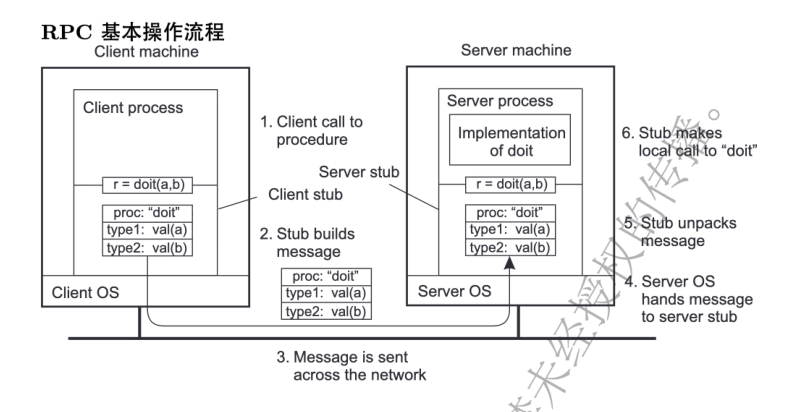
\includegraphics[width=0.8\textwidth]{figures/ch3/ch3_rpc_flow.png}
\end{figure}

（图：RPC 调用流程示意，客户端调用本地过程，由 Stub 封装网络通信，服务端 Stub 调用实际过程并返回结果）

\subsubsection{RPC 的故障语义}

\begin{itemize}
\item \textbf{核心难点}：客户端无法区分“请求未达”与“已处理但应答丢失”。
\item \textbf{常见语义}：
  \begin{itemize}
  \item \textbf{Best-effort}：超时重试，可能重复执行。
  \item \textbf{At-most-once}：绝不重试，保证操作不重复执行。
  \item \textbf{Exactly-once}：[疑似: 可能漏执行]。
  \end{itemize}
\end{itemize}

\section{基于消息的通信}

\subsubsection{Sockets}

\begin{itemize}
\item \textbf{BSD Socket API}：
  \begin{itemize}
  \item 关键操作：\texttt{socket()}, \texttt{bind()}, \texttt{listen()}, \texttt{accept()}, \texttt{connect()}, \texttt{send()}, \texttt{recv()}, \texttt{close()}。
  \item 特点：底层、灵活，但易出错；Client/Server 模式代码结构高度重复。
  \end{itemize}
\end{itemize}

\begin{figure}[htbp]
\centering
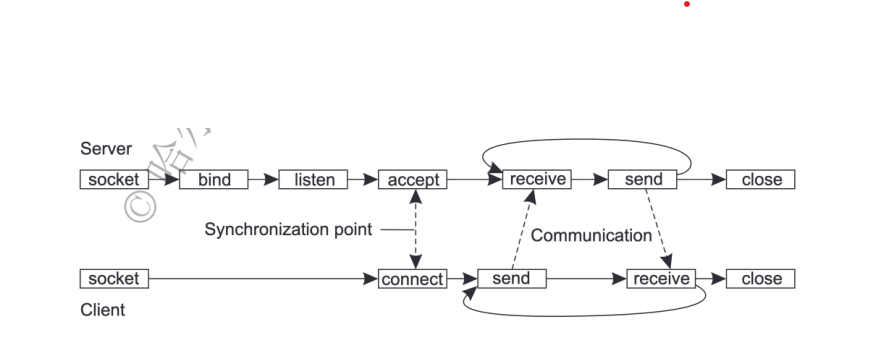
\includegraphics[width=0.8\textwidth]{figures/ch3/ch3_socket_flow.png}
\end{figure}

（图：Socket 通信流程。Server 端依次调用 socket, bind, listen, accept，然后阻塞在 receive；Client 端调用 socket, connect, send，最后 close。）

\textbf{改进}：Golang 等语言对 Socket API 进行了封装，但接收方仍需处理消息边界等问题。

\subsubsection{MOM (Message-Oriented Middleware)}

\begin{itemize}
\item \textbf{基本操作}：
  \begin{itemize}
  \item \textbf{PUT}：将消息追加至指定队列。
  \item \textbf{GET}：阻塞直至队列非空，并取出首消息。
  \item \textbf{POLL}：非阻塞检查并取首消息。
  \item \textbf{NOTIFY}：注册回调，消息到达时触发。
  \end{itemize}
\item \textbf{队列管理器 (Queue Manager)} 管理本地队列。应用仅能访问本地队列，跨节点的通信完全由 MOM 中间件自动完成。
\end{itemize}

\subsubsection{消息代理 (Message Broker)}

\begin{itemize}
\item \textbf{动机}：解决应用间消息格式异构问题。
\item \textbf{核心功能}：
  \begin{itemize}
  \item \textbf{转换 (Transformation)}：在不同协议/数据格式间转换。
  \item \textbf{应用网关 (Application Gateway)}：作为统一入口，提供协议适配、认证鉴权、负载均衡等服务路由。
  \item \textbf{基于主题的路由 (Subject-Based Routing)}：生产者向主题发布消息，消费者按需订阅。
  \end{itemize}
\end{itemize}

\subsubsection{标准协议：AMQP}

\begin{itemize}
\item \textbf{Advanced Message Queuing Protocol}：
  \begin{itemize}
  \item \textbf{基本模型}：
    \begin{itemize}
    \item \textbf{Connection}：稳定连接（TCP 级）。
    \item \textbf{Channel}：单向通道（轻量，可多个）。
    \item \textbf{Session}：会话管理。
    \item \textbf{Link}：基于 Socket，两个单向 Channel 构成。
    \end{itemize}
  \item \textbf{实现示例}：RabbitMQ。
  \end{itemize}
\end{itemize}

\section{组播通信 (Multicast Communication)}

应用层组播 (ALM)：
\begin{itemize}
\item \textbf{思想}：在节点间构建覆盖网络 (overlay network) 实现组播。
\item \textbf{拓扑}：
  \begin{itemize}
  \item 树状 (tree，高效)
  \item 网状 (mesh，需路由)
  \end{itemize}
\item \textbf{指标}：
  \begin{itemize}
  \item \textbf{Link stress}：同一物理链路被 ALM 流的占用情况。
  \item \textbf{Stretch}：ALM 路径延迟 / 物理最短路经延迟。
  \end{itemize}
\end{itemize}

\subsubsection{泛洪 (Flooding) 与优化}

\begin{itemize}
\item \textbf{基本泛洪}：节点向所有邻居广播消息 (除来源外)，且需记录已见消息。
\item \textbf{优化：概率泛洪 (Probabilistic Flooding)}
  \begin{itemize}
  \item 节点以概率 $p_{flood}$ 转发消息。
  \item $p_{flood}$ 可根据度数 (degree) 等动态调整。
  \end{itemize}
\end{itemize}

\subsubsection{Gossip 协议}

\begin{itemize}
\item \textbf{假设}：无写-写冲突。
\item \textbf{特点}：
  \begin{itemize}
  \item 更新操作仅在单个服务端上执行；
  \item 副本仅将更新后的状态传播给少数相邻节点；
  \item 传播是惰性的 (lazy)，即非即时进行；
  \item 最终，每次更新应到达所有副本（最终一致性）。
  \end{itemize}
\item \textbf{副本}：共享同一份数据（或状态）的多个节点实例。
\end{itemize}

\textbf{两类模型}：
\begin{itemize}
\item \textbf{Anti-entropy}：节点随机两两配对，交换状态差值。
\item \textbf{Rumor spreading}：更新节点主动“传染”若干邻居。
\end{itemize}

\subsubsection{Anti-entropy 模型}

\begin{itemize}
\item 节点 $P$ 随机选取系统中另一节点 $Q$，然后执行如下三类操作：
  \begin{itemize}
  \item \textbf{拉取 (Pull)}：$P$ 仅从 $Q$ 拉取其缺失的更新。
  \item \textbf{推送 (Push)}：$P$ 仅将自身新的更新推送给 $Q$。
  \item \textbf{双向 (Push-Pull)}：$P$ 与 $Q$ 互相交换更新。
  \end{itemize}
\item \textbf{性能}：$O(\log N)$ 轮可使全部 $N$ 个节点获知更新。
\item \textbf{概率分析（单源）}：
  \begin{itemize}
  \item Pull: $p_{k+1} = p_k^2$
  \item Push: $p_{k+1} \approx p_k e^{-1}$
  \item Push-pull: $p_{k+1} \approx p_k^3$
  \item 推导见教科书。
  \end{itemize}
  （其中 $p_k$ 为第 $k$ 轮后仍未获知更新的节点比例）
\end{itemize}

\subsubsection{Rumor Spreading 模型}

\begin{itemize}
\item \textbf{机制}：更新者 $s$ 逐个联系其邻居，将更新推送给他们。
\item 设 $s$ 为未知更新节点比例，$1/p_{stop}$ 为停止概率参数。
\item 理论推导可得剩余节点数随时间变化。
\item \textbf{示例}（$N = 10^5$，每次新推送 1 个节点，$p_{stop}=0.2$）：
  \begin{itemize}
  \item 第 1 轮仍有未更新概率：0.203，剩余约 20320 节点。
  \item 第 3 轮仍有未更新概率：0.0198，剩余约 1980 节点。
  \item 第 5 轮仍有未更新概率：0.0025，剩余约 250 节点。
  \item 第 7 轮仍有未更新概率：0.00034，剩余约 34 节点。
  \end{itemize}
\item \textbf{局限}：无法保证 100\% 覆盖，需结合其他机制（如 anti-entropy）。
\end{itemize}

\subsubsection{删除操作的挑战}

\begin{itemize}
\item \textbf{问题}：单纯删除某个值后，Gossip 传播反而可能将其恢复。
\item \textbf{解决方案}：引入\textbf{死亡证书 (death certificate)}。
  \begin{itemize}
  \item 将删除本身视为一种特殊更新，传播至所有副本，且操作必须 [疑似: 覆盖旧数据/具有更高优先级]。
  \end{itemize}
\item \textbf{死亡证书清理策略}：
  \begin{itemize}
  \item \textbf{全局算法}：检测全网已知后统一回收（类似 GC）。
  \item \textbf{乐观策略}：赋予最大生命周期（需承担遗漏风险）。
  \end{itemize}
\end{itemize}

\section{总结}

\begin{itemize}
\item \textbf{通信是分布式系统的基石}，需根据场景选型。
\item \textbf{RPC}：适合请求-应答模式，隐藏网络细节（但需处理故障）。
\item \textbf{Messaging}：适合解耦、异步、可靠投递。
\item \textbf{Multicast / Gossip}：适合大规模状态同步。
\item \textbf{关键原则}：删除操作必须谨慎处理，通常需引入特殊机制。
\end{itemize}

本次课大致对应课程教材第 2 章 [疑似: 第2章]。
